\section{The insertion move for lattice simplices}\label{sec.insert}

Consider a $d$-dimensional lattice simplex $S$ contained in $[0,k]^d$, where $d\geq2$ and $k\geq1$. Let $\mathcal{V}$ be the set of vertices of $S$. For any vertex $u\in\mathcal{V}$, denote by $H_u$ the affine hull of the facet of $\S$ opposite $u$, and by $H_u^-$ the closed half-space of $\mathbb{R}^d$ limited by $H_u$ that does not contain $u$.
For any $v\in\mathcal{V}$, the intersection
\begin{equation}
  C_v=\bigcap_{\substack{u\in\mathcal{V}\\u\neq{v}}}H_u^-
\end{equation}
is a $d$-dimensional cone pointed at $v$. This cone is exactly the set of the points $x\in\mathbb{R}^d$ such that the convex hull of $S\cup\{x\}$ does not admit $v$ as a vertex. By this remark, we have the following lemma.

\begin{lemma}\label{Lem.A}
Let $x$ be a lattice point in $[0,k]^d$. The convex hull of $S\cup\{x\}$ admits $\mathcal{V}\cup{x}$ as its vertex set if and only if $x$ does not belong to $S$ and, for every vertex $v\in\mathcal{V}$, $x$ does not belong to $C_v$.
\end{lemma}

For any $i\in\{1, ..., d\}$, call
$$
\gamma_i^-=\min\{x_i:x\in{S}\}\mbox{ and }\gamma_i^+=\min\{x_i:x\in{S}\}\mbox{.}
$$

Note that, for all $i\in\{1, ..., d\}$, $\gamma_i^-<\gamma_i^+$ because $S$ is $d$-dimensional. The following is the smallest $d$-dimensional combinatorial hypercube containing $S$, whose facets are parallel to the facets of $[0,k]^d$:
$$
Q=\prod_{i=1}^d[\gamma_i^-,\gamma_i^+]
$$

Consider a facet $R$ of $Q$. The intersection of $R$ and $S$ is a non-empty, proper face $F$ of $S$. Since $S$ is a simplex, it admits another non-empty face $F^\star$ whose vertices are exactly the vertices of $S$ that do not belong to $F$.

By construction,
$$
\mathrm{dim}(F)+\mathrm{dim}(F^\star)=d-1\mbox{.}
$$

In particular, there exists a vector $c$ that is orthogonal to both $F$ and $F^\star$. Consider the hyperplane $Y$ of $\mathbb{R}^d$ that admits $c$ as a normal vector and such that $F^\star\subset{Y}$. The intersection $S\cap{Y}$ is precisely $F^\star$. Denote by $Y^-$ the closed half-space of $\mathbb{R}^d$ bounded by $Y$ that does not contain $F$. In the statement of the following lemma, $\mathrm{aff}(F)$ denotes the affine hull of $F$.

\begin{lemma}\label{Lem.B}
Consider a vertex $v$ of $S$.
\begin{itemize}
\item[i.] If $v$ is a vertex of $F$, then $C_v\cap{Q}$ is a subset of $\mathrm{aff}(F)$,
\item[ii.] If $v$ is a vertex of $F^\star$, then $C_v$ is a subset of $Y^-$.
\end{itemize}
\end{lemma}

\begin{proof}
First observe that, if $s$ is a face of $S$ and $H$ is a hyperplane of $\mathbb{R}^d$ that intersects $S$ exactly along $s$, then
$$
\bigcap_{\substack{u\in\mathcal{V}\\u\not\in{s}}}H_u^-\subset{H^-}\mbox{,}
$$
where $H^-$ is the closed half space of $\mathbb{R}^d$ bounded by $H$ and disjoint from the interior of $S$. Further observe that the intersection of $H$ with
$$
\bigcap_{\substack{u\in\mathcal{V}\\u\not\in{s}}}H_u^-
$$
is precisely the affine hull of $s$. Taking $s=F$ and $H=\mathrm{aff}(R)$, one obtains that for any vertex $v$ of $F$, $C_v\cap{Q}$ is a subset of $\mathrm{aff}(F)$. Taking $s=F^\star$, and $H=Y$, ones obtains that, for any vertex $v$ of $F^\star$, $C_v$ is a subset of $Y^-$.% The result therefore holds because any vertex of $\S$ is either a vertex of $F$ or a vertex of $F^\star$.
\end{proof}

As an immediate consequence of this and Lemma \ref{Lem.A}, for any lattice point $x\in[0,k]^d$ that does not belong to the affine hull of $F$, or to $Y^-$, the convex hull of $S\cup\{x\}$ admits, as vertices, $x$ and all the vertices of $S$.

Assume, without loss of generality that $c$ has norm $1$ and that it points towards $Y^-$. Observe that the intersection of $[0,k]^d$ with the affine hull of $R$ is a $(d-1)$-dimensional cube. Denote
\begin{equation}\label{eq.A}
\delta=\min\{c\mathord{\cdot}x:x\in\mathrm{aff}(R)\cap[0,k]^d\}\mbox{.}
\end{equation}

The set
$$
G=\{x\in\mathrm{aff}(R)\cap[0,k]^d:c\mathord{\cdot}x=\delta\}
$$
is a face of $\mathrm{aff}(R)\cap[0,k]^d$. It follows that $G$ is a cube of dimension at most $d-1$. Recall that $c$ is orthogonal to both $F$ and $F^\star$. As a consequence, the map $x\mapsto{c\mathord{\cdot}x}$ is constant within $F$ and within $F^\star$. Call $\varepsilon$ the value of $c\mathord{\cdot}x$ when $x\in{F}$ and $\varepsilon^\star$ the value of $c\mathord{\cdot}x$ when $x\in{F^\star}$. Since $F$ and $Y^-$ are disjoint, $\varepsilon<\varepsilon^\star$. Moreover, by (\ref{eq.A}), $\delta\leq\varepsilon$. Observe that the latter inequality is strict if and only if $F$ is not a subset of $G$. In this case, $F$, $G$, and $Y$ belong to distinct parallel hyperplanes and we immediately obtain the following.
\begin{lemma}\label{Lem.BC}
If $F\not\subset{G}$ then $G$ is disjoint from both $\mathrm{aff}(F)$ and $Y^-$.
\end{lemma}

If, on the contrary, $\delta$ and $\varepsilon$ coincide, then $F\subset{G}$. This situation is familiar: we are looking at a lattice simplex $F$ contained in a (possibly degenerate) lattice cube $G$. If the dimension of $G$ is greater than the dimension of $F$, then the following lemma provides the desired result.

\begin{lemma}\label{Lem.C}
If $k$ and $d$ are positive and if $P$ is a lattice $(d,k)$-polytope of dimension less than $d$ then there exists a lattice point $x$ that belongs to $[0,k]^d$ but that does not belong to the affine hull of $P$.
\end{lemma}
\begin{proof}
If $P$ is a lattice $(d,k)$-polytope of dimension less than $d$, then the intersection $I$ of its affine hull with $[0,k]^d$ cannot contain more than $(k+1)^{d-1}$ lattice points. Indeed, one can always project $I$ orthogonally on a facet of $[0,k]^d$ in such a way that the dimension of the projection is not less than that of $I$. Such a projection induces an injection from the lattice points in $I$ into the lattice points in the facet on which the projection is made.

Now observe that $[0,k]^d$ contains $(k+1)^d$ lattice points. Since $k$ is positive, $(k+1)^{d-1}<(k+1)^d$ and the lemma is proven.
\end{proof}

We now have to address the case when, regardless of which facet $R$ of $Q$ is chosen, $F$ is a subset of $G$ and these polytopes have the same dimension.

\begin{lemma}\label{Lem.EA}
Call $g$ the maximal dimension of $F$ over all the possible choices of the facet $R$ among the facets of $Q$. Assume that, for any choice of $R$ among the facets of $Q$, $G$ admits $F$ as a subset and the dimensions of $F$ and $G$ coincide. If the difference $d-g$ is not less than $2$, then for some choice of $R$ such that $F$ has dimension $g$, there exists a lattice point in $R\mathord{\setminus}[\mathrm{aff}(F)\cup{Y^-}]$.
\end{lemma}
\begin{proof}
Consider a facet $R$ of $Q$ such that $F$ has dimension exactly $g$. As $G$ admits $F$ as a subset, $G$ must be a face of $Q$. By the maximality of $g$, the intersection of $S$ with any facet of $Q$ incident to $G$ is precisely $F$. In other words, $G$, $F$, $F^\star$, $Y$, and $c$ do not depend on which facet $R$ of $Q$ is chosen, provided this facet is incident to $G$. As a consequence, and taking advantage of the symmetries of the cube, one can choose $R$ in such a way that all the coordinates of $c$ are non-negative, the largest coordinate of $c$ is $c_1$, and
$$
R=\{x\in{Q}:x_1=\gamma_1^-\}\mbox{.}
$$

Recall that $F^\star$ is non-empty and consider a vertex $v$ of $F^\star$. By the definition of $\varepsilon^\star$, we have:
$$
\sum_{i=1}^dc_iv_i=\varepsilon^\star\mbox{.}
$$

This equality can be transformed into
$$
c_1\gamma_1^-+\sum_{i=2}^dc_iv_i=\varepsilon^\star-c_1(v_1-\gamma_1^-)\mbox{.}
$$

In other words, the orthogonal projection $w$ of $v$ on $R$ (whose coordinates coincide with the coordinates of $v$, except for the first coordinate that is equal to $\gamma_1^-$ instead of $v_1$) satisfies $c\mathord{\cdot}w=\varepsilon^\star-c_1(v_1-\gamma_1^-)$. As $c_1$ is non-zero and as $v_1>\gamma_1^-$, we obtain $c\mathord{\cdot}w<\varepsilon^\star$. It immediately follows that $w\not\in{Y^-}$. Now assume that $d-g$ is at least $2$. In this case, $G$ is the intersection of at least two facets of $Q$. Since $v$ does not belong to any of the facets of $Q$ that contain $G$, then $w$ cannot belong to $G$. As a consequence $w$ does not belong to the affine hull of $F$. By construction, $w$ is a lattice point, and the lemma is proven.
\end{proof}

\begin{theorem}\label{thm.add}
Call $g$ the maximal dimension of $F$ over all the possible choices of the facet $R$ among the facets of $Q$. If $d-g$ is not less than $2$, then one can choose the facet $R$ among the facets of $Q$ in such a way that $F$ has dimension $g$ and, for some lattice point $x$ in $R$, the convex hull of $S\cup\{x\}$ admits $\mathcal{V}\cup\{x\}$ as its vertex set, and the convex hull of $F\cup\{x\}$ is a simplex.
\end{theorem}

\begin{proof}
Assume that $g$ is at most $d-2$. If $R$ can be chosen among the facets of $Q$ in such a way that $F\not\subset{G}$, then let $R$ be any such facet and $x$ a lattice point in $G$. By Lemma \ref{Lem.BC}, $x$ cannot belong to the affine hull of $F$. In particular, the convex hull of $F\cup\{x\}$ is a simplex. Moreover, $x$ does not belong to $Y^-$ either. Hence, by Lemmas \ref{Lem.A}, and \ref{Lem.B}, the convex hull of $S\cup\{x\}$ admits $\mathcal{V}\cup\{x\}$ as its vertex set.

Now assume that for any choice of $R$ among the facets of $Q$, $F\subset{G}$ but $R$ can be chosen such that the dimension of $F$ is less than the dimension of $G$. In this case, by Lemma \ref{Lem.C}, there exists a lattice point $x$ in $G$ that does not belong to the affine hull of $F$. In particular, the convex hull of $F\cup\{x\}$ is a simplex. As in addition, $Y^-$ is disjoint from $G$, it follows from Lemmas \ref{Lem.A}, and \ref{Lem.B} that the convex hull of $S\cup\{x\}$ admits $\mathcal{V}\cup\{x\}$ as its vertex set.

Finally, assume that for any choice of $R$ among the facets of $Q$, $F$ is a subset of $G$ and the dimensions of $F$ and $G$ coincide. By Lemma \ref{Lem.EA}, one can choose $R$ such that $F$ has dimension $g$ and there exists a lattice point in $R$ that does not belong to the affine hull of $F$ or to $Y^-$. In this case, the convex hull of $F\cup\{x\}$ is a simplex and, by Lemmas \ref{Lem.A}, and \ref{Lem.B}, the convex hull of $S\cup\{x\}$ admits $\mathcal{V}\cup\{x\}$ as its vertex set, which completes the proof.
\end{proof}

The following corollary shows that an insertion move is possible for $S$ on at least one lattice point. The argument in this proof will be used again in the next section, in order to prove that $\Gamma(d,k)$ is always connected.

\begin{corollary}\label{cor.add}
There exists a lattice point $x$ in $[0,k]^d$ such that the convex hull of $S\cup\{x\}$ admits $\mathcal{V}\cup\{x\}$ as its vertex set.
\end{corollary}
\begin{proof}
If, for any possible choice of $R$ among the facets of $Q$, the dimension of $F$ is at most $d-2$, then the result follows from Theorem \ref{thm.add}. Assume that, for some facet $R$ of $Q$, $F$ has dimension $d-1$. In this case, $Y$ is parallel to $R$ and $F^\star$ is made up of a single vertex, say $v$. By the same argument as in the proof of Lemma \ref{Lem.B}, the intersection of $C_v$ with $Y$ is precisely $v$ and, for every vertex $u$ of $F$, $C_u$ is disjoint from $Y$. Hence, by Lemma \ref{Lem.A}, any lattice point $x$ in $Y\cap[0,k]^d$ distinct from $v$ is such that the convex hull of $S\cup\{x\}$ admits $\mathcal{V}\cup\{x\}$ as its vertex set. As $k\geq1$, there exists at least one such lattice point.
\end{proof}

\section{The connectivity of $\Gamma(d,k)$}\label{sec.conect}

We first prove in this section that $\Gamma(2,k)$ is a connected graph. This will serve as the base case for the inductive proof that $\Gamma(d,k)$ is connected. In the whole section, we call \emph{corner simplex} of $[0,k]^d$ the simplex whose vertices are the origin (the lattice point whose all coordinates are zero), and the $d$ lattice points in $[0,k]^d$ distant from the origin by exactly $1$.

\begin{theorem}\label{thm.Connec2}
For any positive $k$, $\Gamma(2,k)$ is connected.
\end{theorem}
\begin{proof}
Consider a lattice polygon $P$ contained in the square $[0,k]^2$. First observe that, if $P$ is not a simplex, then a deletion move can always be performed for some vertex of $P$. In particular, $P$ can always be transformed into a lattice triangle by a sequence of deletions. Hence, in order to prove the theorem, we only need to show the connectedness of the subgraph of $\Gamma(2,k)$ induced by triangles and quadrilaterals. Consider a lattice triangle contained in the square $[0,k]^2$. If this triangle does not have a horizontal or a vertical edge then, by Theorem \ref{thm.add}, an insertion move can be performed to transform it into a quadrilateral with a horizontal or a vertical edge, say $e$. It is then possible to perform a deletion move on one of the vertex of  this quadrilateral that is not incident to $e$ in order to obtain a triangle $T$ that admits $e$ as an edge. The strategy is then to transform $T$ into the corner triangle of $[0,k]^2$ using the sequence of moves sketched in Fig. \ref{fig:connect}. This figure shows the case when $e$ is the horizontal edge on the bottom of $T$. In each portion of the figure, the next point on which a move will be performed is colored blue. First observe that an insertion move can be performed on a lattice point in the line parallel to $e$ that contains the vertex of $T$ opposite $e$ in order to obtain a quadrilateral with three horizontal or vertical edges as shown in Figs. \ref{fig:connect}(i) and \ref{fig:connect}(ii).
\begin{figure}[b]
\begin{center}
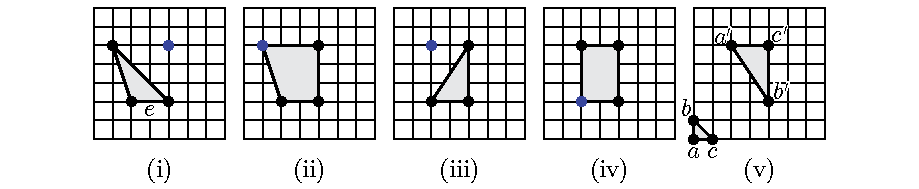
\includegraphics[width=\textwidth]{../assets/connect}
\caption{An illustration of the sequence of deletion and insertion moves from the lattice triangle in (i) to the corner triangle on the bottom-left of (v).}
\label{fig:connect}
\end{center}
\end{figure}
A deletion move on one of the vertices of the quadrilateral then results in a triangle with a horizontal and a vertical edge shown in Fig. \ref{fig:connect}(iii). After that, the triangle has a unique oblique edge that faces one of the four vertices of the square $[0,k]^2$. It is always possible to make this edge face the vertex on the bottom left of the square by performing an insertion move to obtain a rectangle and then a deletion move on the bottom-left vertex of the rectangle. This sequence of moves is illustrated in Figs. \ref{fig:connect}(iii) and \ref{fig:connect}(iv) in the case when the oblique edge initially faces the top left vertex. Finally, one can transform the resulting triangle into the corner triangle of $[0,k]^2$ by inserting the vertices labeled $a$, $b$, and $c$ in Fig. \ref{fig:connect}(v) in this order, the insertion of $x$ being immediately followed by the deletion of $x'$.
\end{proof}

\begin{theorem}\label{lem.Connecd}
For any $d\geq2$ and any positive $k$, $\Gamma(d,k)$ is connected.
\end{theorem}
\begin{proof}
The proof proceeds by induction on $d$. The base case is provided by Theorem \ref{thm.Connec2}. Again, one can always transform a $d$-dimensional lattice $(d,k)$ polytope into a $d$-dimensional simplex by a sequence of deletion moves. Therefore, we only need to prove that the subgraph induced in $\Gamma(d,k)$ by simplices and by polytopes with $d+2$ vertices is connected. The strategy will be, again, to transform any simplex in this graph into the corner simplex of $[0,k]^d$.

Assume that $d\geq3$, consider a lattice simplex $S$ contained in $[0,k]^d$, and call $\mathcal{V}$ the vertex set of $S$. For any $i\in\{1, ..., d\}$, call
$$
\gamma_i^-=\min\{x_i:x\in{S}\}\mbox{ and }\gamma_i^+=\min\{x_i:x\in{S}\}\mbox{.}
$$

Further denote
$$
Q=\prod_{i=1}^d[\gamma_i^-,\gamma_i^+]\mbox{.}
$$

Call $g$ the maximal dimension of the intersection of $S$ and a facet of $Q$. If $g$ is at most $d-2$ then, by Theorem \ref{thm.add}, there exists a facet $R$ of $Q$ such that $S\cap{R}$ is $g$-dimensional and a lattice point $x\in{R}$ such that the convex hull of $S\cup\{x\}$ admits $\mathcal{V}\cup\{x\}$ as its vertex set and the convex hull of $[S\cap{R}]\cup\{x\}$ is a simplex. In other words, one can perform an insertion move on vertex $x$ to transform $S$ into a polytope with vertex set $\mathcal{V}\cup\{x\}$. Since the convex hull of $S\cup\{x\}$ is a simplex, one can find a simplex whose vertex set contains all the vertices of $S\cup\{x\}$, and is a subset of $\mathcal{V}\cup\{x\}$. This simplex can be obtained from the convex hull of $\mathcal{V}\cup\{x\}$ by a single deletion move. Now observe that the intersection of this simplex with $R$ has dimension $g+1$. Repeating this procedure provides a sequence of insertion and deletion moves that transform $S$ into a lattice simplex whose intersection $F$ with a facet $R$ of $Q$ has dimension $d-1$. Call $v$ the unique vertex of the lattice simplex that does not belong to $R$. In other words, this lattice simplex is a pyramid with apex $v$ over $F$. Observe that, in this case, any sequence of insertion and deletion moves that can be performed for $F$ within the cube $\mathrm{aff}(R)\cap[0,k]^d$ can also be performed within $[0,k]^d$ for the pyramid with apex $v$ over $F$. By induction, one can transform $F$ into any lattice simplex in $\mathrm{aff}(R)\cap[0,k]^d$ by a sequence of deletion and insertion moves. Therefore, we can build a sequence of moves that transform $S$ into the $d$-dimensional lattice simplex $S'$ whose vertex set is made up of $v$, of the lattice point $w$ in $\mathrm{aff}(R)\cap[0,k]^d$ with a unique non-zero coordinate, and of the $d-1$ lattice points in $\mathrm{aff}(R)\cap[0,k]^d$ distant by exactly $1$ from $w$.

Now observe that one can perform an insertion move on any lattice vertex distinct from $v$ in the intersection of $[0,k]^d$ with the hyperplane parallel to $R$ that contains $v$. We proceed by inserting the lattice point in this intersection whose orthogonal projection on $R$ is $w$ and then, by deleting $v$. Calling $v'$ any of the $d-1$ lattice points in $\mathrm{aff}(R)\cap[0,k]^d$ distant from $w$ by exactly $1$, the simplex that results from the latter deletion is a pyramid with apex $v'$ over a $(d-1)$-dimensional simplex $F'$ such that, for some $i\in\{1, ..., d\}$, $v'$ satisfies $v'_i=1$ and every vertex $u$ of $F'$ satisfies $u_i=0$. Call $R'$ the facet of $[0,k]^d$ made up of the points $x$ such that $x_i=0$. By induction, one can transform $F'$ within $R'$ into the corner simplex of $R'$. From there, one can perform an insertion move on any lattice vertex distinct from $v'$ in the intersection of $[0,k]^d$ with the hyperplane parallel to $R'$ that contains $v'$. We proceed by inserting the lattice point in this intersection whose orthogonal projection on $R'$ is the origin. Since $v'_i=1$, the $i$-th coordinate of the inserted point is $1$, and its other coordinates are all equal to $0$. Hence, after a last deletion move on $v'$, the resulting simplex is the corner simplex of $[0,k]^d$, as desired.
\end{proof}

\clearpage
 \section{Additional experiments}\label{Sec.Tab}

%% % summary table
%% \begin{table}[h]
%%   \begin{center}
%%   \begin{tabular}{c|r|r|r|r|r|r}
%%     & \multicolumn{2}{c|}{$1000$ steps} & \multicolumn{2}{c|}{$10000$ steps} & \multicolumn{2}{c}{$100000$ steps} \\
%%     \hline
%%     \hline
%%     $k$ & vertices & volume & vertices & volume & vertices & volume \\
%%     \hline
%%     $3$ & $4.798$ & $4.148$ & $4.734$ & 4.353 & 4.711 & 4.343\\
%%     $4$ & $5.38$ & $7.754$ & $5.288$ & 7.349 & 5.266 & 7.314\\
%%     $5$ & $6.068$ & $11.844$ & 6.003 & 11.580 & 5.868 & 11.331\\
%%     $6$ & $6.93$ & $14.934$ & 6.520 & 17.144 & 6.540 & 16.933\\
%%     $7$ & $7.031$ & $21.050$ & 7.198 & 23.210 & 7.235 & 23.925\\
%%     $8$ & $7.157$ & $25.922$ & 7.979 & 33.357 & 7.856 & 33.667\\
%%     $9$ & $8.558$ & $33.712$ & 8.3741 & 44.350 & 8.418 & 41.563\\
%%     $10$ & $8.736$ & $43.375$ & 8.943 & 55.423 & 9.136 & 56.358\\
%%     $15$ & $10.483$ & $125.405$ & 11.462 & 101.626 & 11.517 & 137.427\\
%%     $20$ & $13.07$ & $209.562$ & 14.170 & 219.586 & 13.929 & 246.689\\
%%     $25$ & $12.695$ & $314.633$ & 15.829 & 376.770 & 16.669 & 374.121\\
%%     $30$ & $13.501$ & $356.220$ & 16.835 & 532.784 & 18.165 & 585.092\\
%%     $40$ & $14.904$ & $365.466$ & 20.393 & 714.765 & 22.618 & 855.234\\
%%     $50$ & $18.875$ & $369.500$ & 21.639 & 816.006 & 25.351 & 1779.055\\
%%     $60$ & 18.813 & 542.450 & 20.51 & 1112.126 & 27.56 & 2337.680\\
%%     $70$ & 17.534 & 525.187 & 21.804 & 1271.738 & 31.058 & 3022.452\\
%%     $80$ & 18.8 & 593.20 & 24.999 & 1547.383 & 32.995 & 3343.108\\
%%     $90$ & 19.771 & 562.75 & 24.240 & 1499.416 & 33.903 & 3728.283\\
%%     \hline
%%   \end{tabular}
%%   \caption{A summary of measures on the number of vertices and volume of convex polygon visited in a long walk on the Markov chain, for a selection values of $k$ and for $1000$, $10000$ and $100000$ steps walks.}
%%   \label{Tab.Summary}
%%   \end{center}
%% \end{table}

%% \begin{figure}[h]
%%   \centering
%%   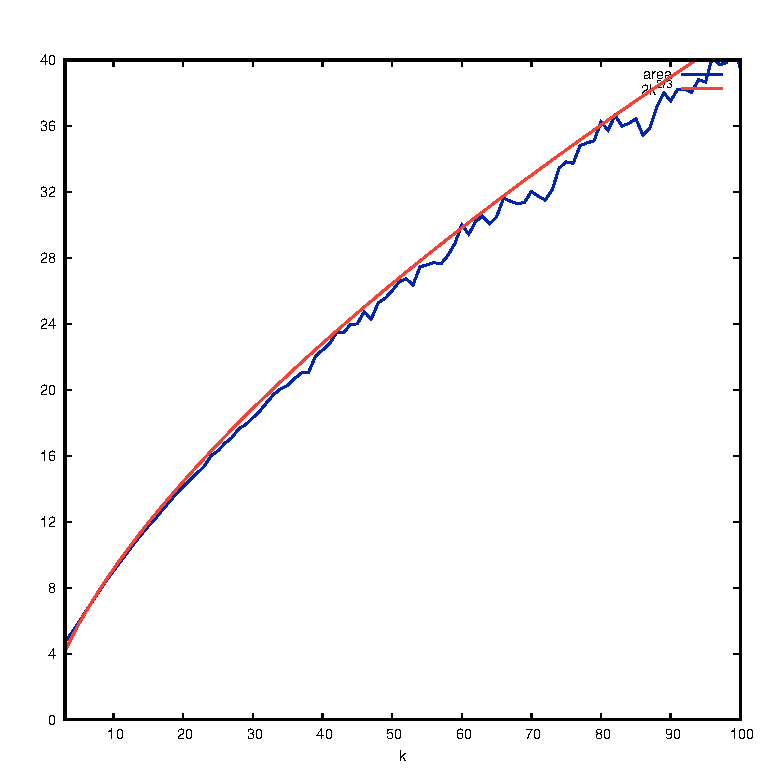
\includegraphics[scale=0.7]{npoint_lim}
%%   \caption{The blue curve shows the verage number of vertices of a polygon in a 1 million steps run, whereas the red one is $2k^{2/3}$.}
%%   \label{Fig.Nlim}
%% \end{figure}

%% \begin{figure}[h]
%%   \centering
%%   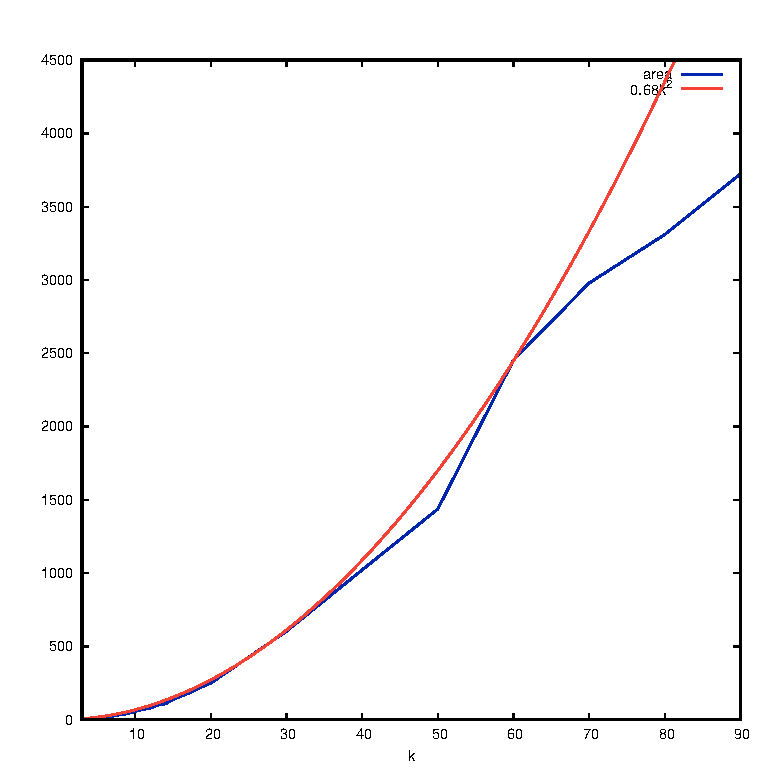
\includegraphics[scale=0.7]{volume_lim}
%%   \caption{The blue curve shows the average area of a polygon in a 1 million steps run, whereas the red one is $0.68k^2$.}
%%   \label{Fig.Vlim}
%% \end{figure}



\begin{figure}[h!]
  \centering
  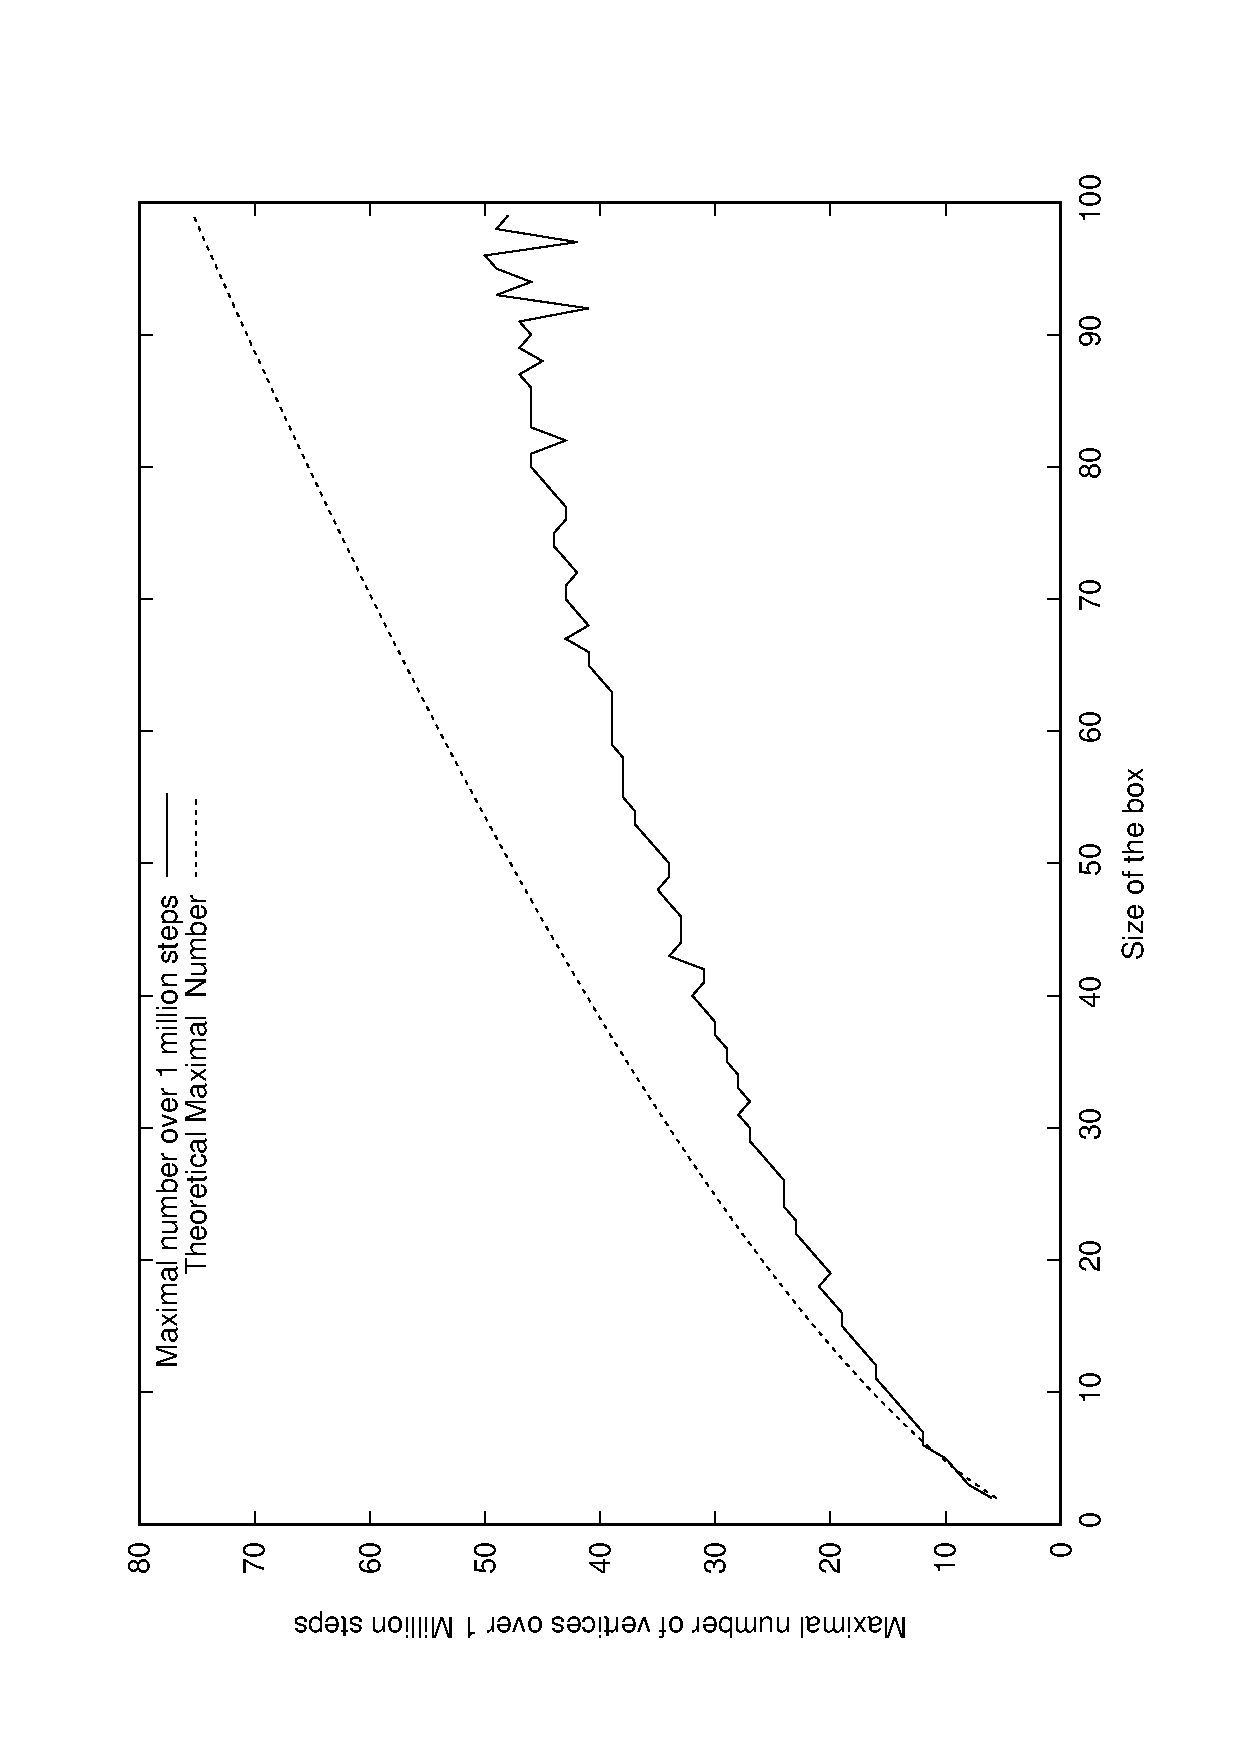
\includegraphics[scale=0.3]{max1M}
  \caption{The average over $100$ runs of the maximal number of vertices of the visited polygons over $1$ million step walks and the theoretical maximum number of vertices of a lattice polygon contained in $[0,k]^2$.}
  \label{Fig.Nlim}
\end{figure}
\begin{figure}[h!]
  \centering
  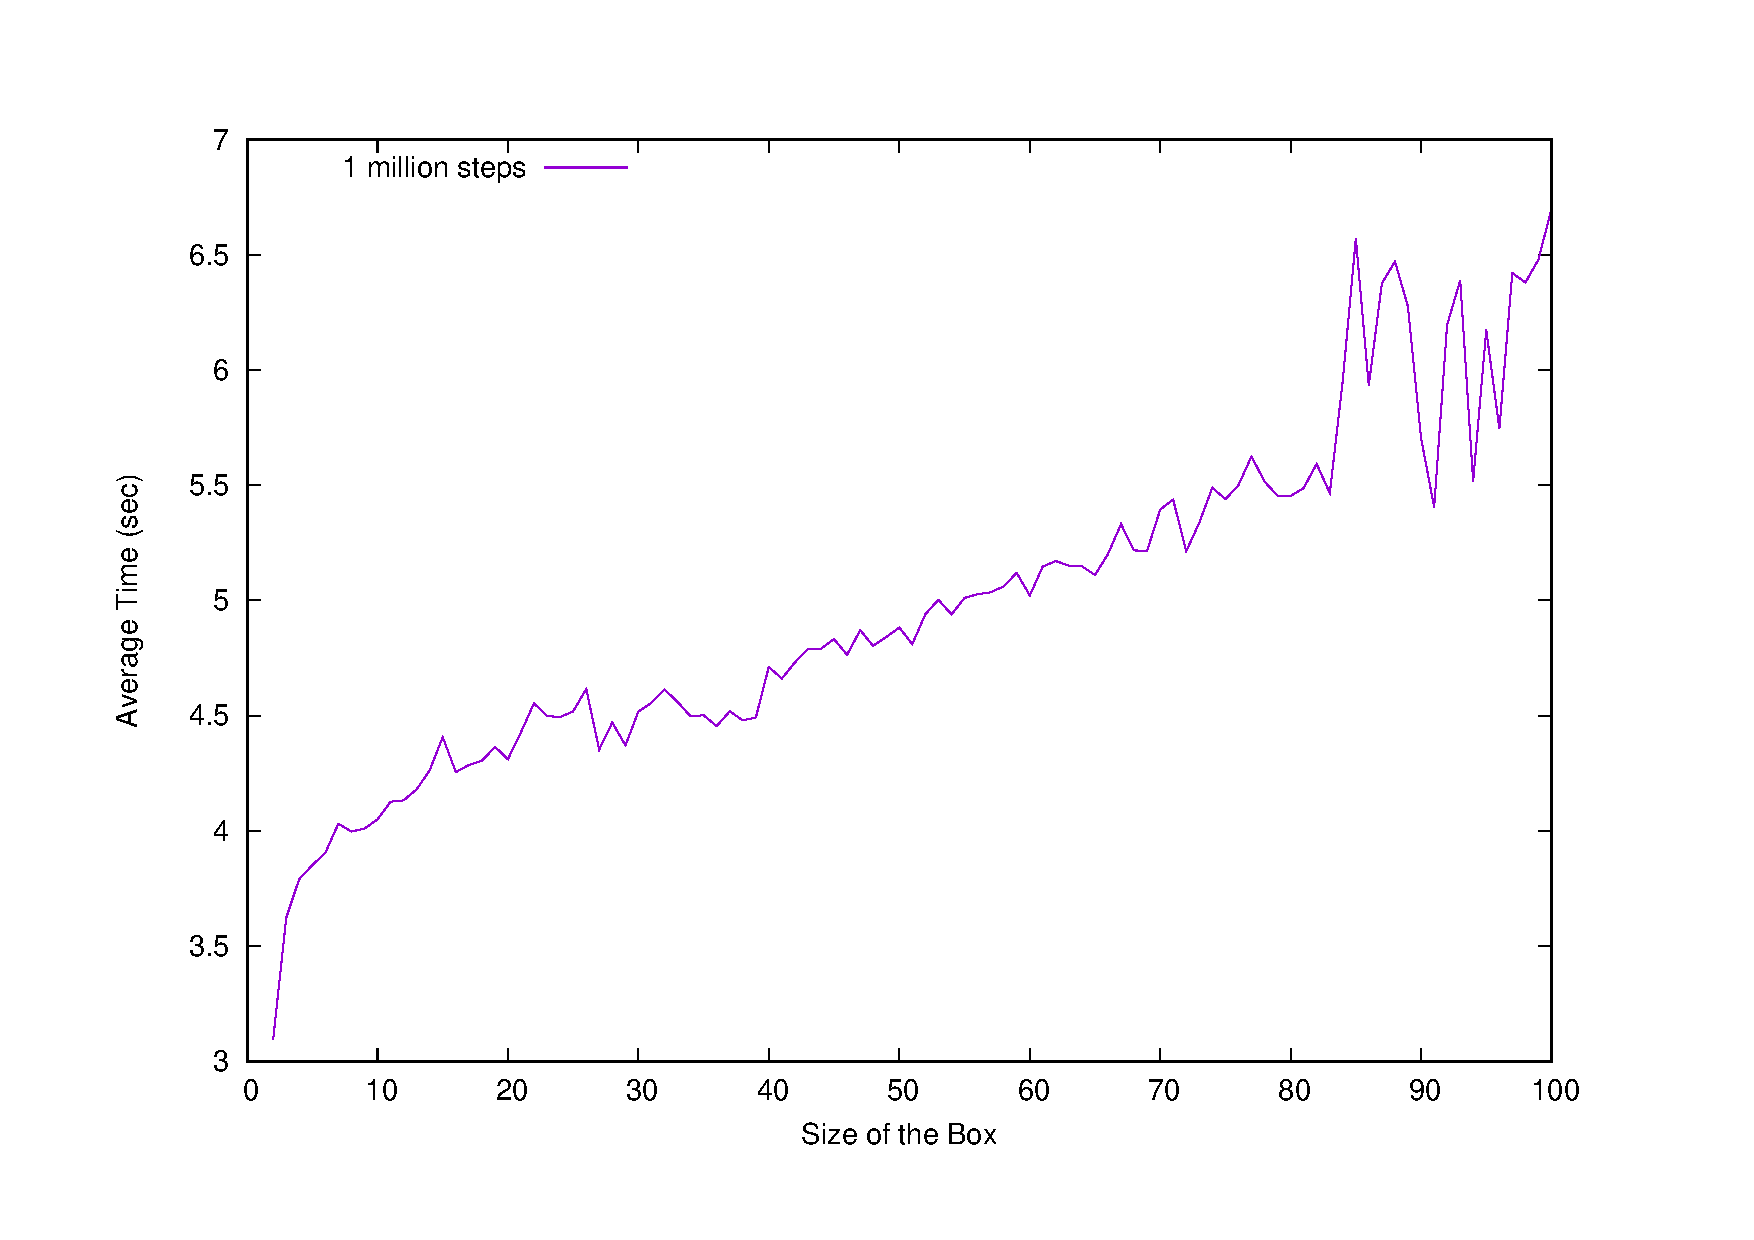
\includegraphics[scale=0.3]{averageTime}
  \caption{The average over $10$ runs, of the time in seconds needed to perform a $1$ million steps walk.}
  \label{Fig.Nlim}
\end{figure}

